%%%%%%%%%%%%%%%%%%%%%%%%%%%%%%%%%%%%%%%%%%%%%%%%%%%%%%%%%%%%%%%%%%%%%%%%%%%%%%%%

\begin{frame}[fragile]{Cover tree run times}

%\begin{tikzpicture}
%\node at (0,2) {
    %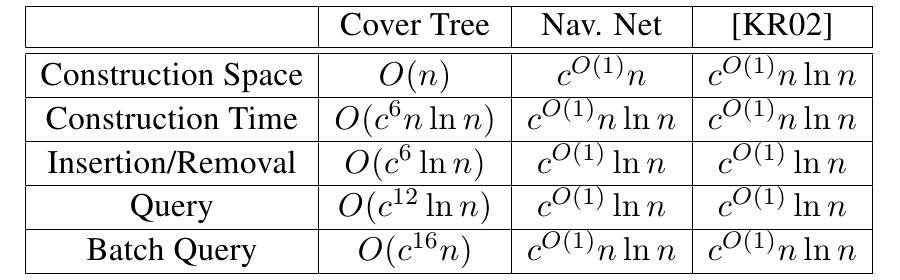
\includegraphics[width=12cm]{covertree/runtimes}

\begingroup
\begin{center}
\renewcommand*{\arraystretch}{1.9}
\begin{tabular}{l|c|c|}
& \footnotesize My Dissertation
& \footnotesize Beygelzimer \emph{et. al.}, 2006
\\
\hline
Number of nodes       & $n$                   & $O(n)$                \\
%Construction time     & $O(\cdoub^3n\log n$   & $O(\cexp^6 n\log n)$  \\
Insertion time (1 pt) & $O(\cdoub^3 \log n)$   & $O(\cexp^6 \log n)$   \\
Query time ~~~(1 pt)  & $O(\chole^4\log n)$    & $O(\cexp^{12}\log n)$ \\
%Query time ~~~(n pts) &  --                 & $\cexp^{16} n$     \\
\hline
\end{tabular}
\end{center}
\endgroup

\ignore{
{\footnotesize
    \begin{tabular}{>\centering m{2cm}|>\centering m{2.0cm}|>\centering m{2.0cm}|>\centering m{2.0cm}|c|}
    %\cline{2-5}
    & \multicolumn{2}{c|}{Cover Tree}
    %& Cover Tree
    & \footnotesize Nav. Net
    & \footnotesize Met. Skip List
    %& \footnotesize Ball Tree
    \\
    \cline{2-5}
    & \footnotesize My Dissertation
    & \footnotesize Beygelzimer ~~~\emph{et. al.}, 2006
    & \footnotesize Krauthgamer and Lee, 2004
    %& \footnotesize Karger and Ruhl, 2002
    & \begin{tabular}{c}
        Karger and\\
        Ruhl, 2002
      \end{tabular}
    %& \begin{tabular}{c}
        %Omohundro,\\
        %1989
      %\end{tabular}
    \\
    \hline
    Construction space    & $n$                 & $n$                & $\poly{\cexp}n$           & $\poly{\cexp}n \log n$    \\%& $n$ \\
    Construction time     & $\cdoub^3n\log n$   & $\cexp^6 n\log n$  & $\poly{\cexp}n\log n$     & $\poly{\cexp}n \log n$    \\%& $n^2$ \\
    Insertion time (1 pt) & $\cdoub^3 \log n$   & $\cexp^6 \log n$   & $\poly{\cexp}\log n$      & $\poly{\cexp} \log n$     \\%& $n$ \\
    Query time ~~~(1 pt)  & $\chole^4\log n$    & $\cexp^{12}\log n$ & $\poly{\cexp}\log n$      & $\poly{\cexp} \log n$     \\%& $n$\\
    Query time ~~~(n pts) &  --                 & $\cexp^{16} n$     & $\poly{\cexp}n\log n$     & $\poly{\cexp}n \log n$    \\%& $n^2$\\
    \hline

    \end{tabular}
}
}
%};

\vspace{0.15in}
The variables $\cdoub\approx\chole\approx\cexp$ measure the ``intrinsic dimension'' 

\vspace{0.15in}
%\footnotesize
%\node at (-1,-0.4) { (Beygelzimer \emph{et. al.}, 2006)};
%\node at (2,-1) { (Krauthgamer and Lee, 2004)};
%\node at (4,-0.4) { (Karger and Ruhl, 2002) };
%\draw[->] (-1,-0.25) -- (-0.9,0.1);
%\draw[->] (1.3,-0.75) -- (1.5,0.1);
%\end{tikzpicture}

%Karger and Ruhl, Symposium on the Theory of Computing, 2002
%
%\vspace{0.15in}
%Krauthgamer and Lee, Symposium on Discrete Algorithms, 2004
%
%\vspace{0.15in}
%Beygelzimer, Kakade, and Langford, ICML, 2006

\vspace{0.05in}
Recent research either:
\begin{itemize}
\item Extends the analysis on cover trees {\footnotesize (Ram \emph{et. al.}, 2010; Curtin \emph{et. al.}, 2015)}
\item Focuses on \emph{approximate} queries (too many papers to list)
\end{itemize}

%\vspace{0.15in}
%More recent research focuses on \emph{approximate} queries: LHS, Spill trees
%\textbf{open problem}: construct a data structure in time $O(c^{O(1)}n)$ for some dimensionality $c$; is it even possible?
%\vspace{0.15in}

\end{frame}

